\documentclass[a4paper]{article}

\usepackage[english]{babel}
\usepackage[utf8]{inputenc}
\usepackage{amsmath}
\usepackage{graphicx}
\usepackage[colorinlistoftodos]{todonotes}

\title{Electric Circuits 307:
Single Transistor Circuits II}

\author{Josh Lofy}

\date{11/21/2014}

\begin{document}
\maketitle

\begin{abstract}
We designed two different kinds of switches using either a bipolar or MOSFET transistor.  We then confirmed current and voltage readings measured from the designed switches using theoretical circuits on MultiSim v10.1.  
\end{abstract}

\section{Introduction}

In this lab our group designed two different kinds of switches.  Our group made 4 separate circuits, two of which would use a mechanical switch and two of which used a function generator with a specific offset to act as if a DC source 

\[0<Volts<V\]

There were two different transistors used: A bipolar transistor (2N4401) and a MOSFET transistor (IRF510).  Each transistor had one mechancical switch circuit and one with the frequency generator.

To see that our circuit was working we used an LED, an analog Ammeter, and the osciloscope.  The LED showed, very quickly, wheter our circuit was functioning or not.  The analog Ammeter we used was able to show current running through the diode similar to that of theoretical circuit in MultiSim v10.1.  And finally, the oscilloscope showed that the signal being sent into the gate was what was turning our switch on.

\section{Circuit Design}

\subsection{Materials required}

\begin{itemize}
\item 10k Ohm Resistor
\item 1k Ohm Resistor
\item Oscilioscope
\item Function generator
\item DC power Source
\item Mechanical switch
\item 2N4400 Transistor
\item IRF510
\item LED
\item Ammeter (mA)
\end{itemize}

\subsection{Bipolar Transistor Circuit ~ 2N4400}

My group was able to measure the current running through the LED using a analog ammeter for this circuit.  In MultiSim v10.1 our circuit created a current of 5.88mA.  Using the analog meter, we saw 6mA of current.  We could also visibly see the LED turn on and off when power was applied through the switch.  

This circuit was created once using a mechanical switch, and once with the function generator.  Both worked well, and we were able to find a acceptable signal out of them.  For the design with theoretical output, view Figure 1.

\begin{figure}
\centering
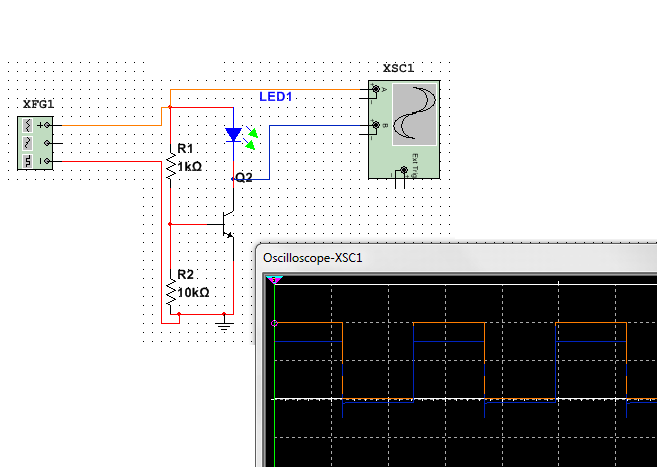
\includegraphics[width=.5\textwidth]{Circuit_one.png}
\caption{\label{fig:Circuit_one}Bipolar transistor circuit with theoretical Osciloscope output - MultiSim Blue v13}
\end{figure}

\subsection{MOSFET Power Transistor Circuit ~ IRF510}

The group was able to create a MOSFET power switch using the function generator, but we ran into too many obstacles while setting up the mechanical switch.  We did attempt the circuit, but were unable to reproduce it sufficently.  This is because there were too many wires going between the mechanical switch and the circuit, making it difficult for the switch to move and connnector to the circuit properly.

The signal we were able to measure agreed with our expected signal through the osciloscope with the MOSFET transistor and a function generator.  Using the osciloscope in conjunction with the LED in our circuit (See Figure 2) we were able to make sure the values matched the theoretical values from MultiSim v10.1.


\begin{figure}
\centering
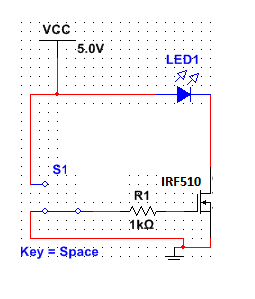
\includegraphics[width=.5\textwidth]{Circuit_two.png}
\caption{\label{fig:Circuit_two}MOSFET power transistor circuit with set up with a mechanical switch - MultiSim Blue v13}
\end{figure}

\section{Conclusion}

Our switches were able to function both as mechanical and frequency switches with \todo{With some physical exceptions due to poor design} very few obstacles.  We were able to see the effectively how power MOSFETs use a voltage at their gate to control the signal traveling from the drain to the source.  In this case, our signal we transmitted was only a DC voltage, but it would be possible to turn on and off a more complicated signal going out to a larger part of the circuit.  These concepts are important when we begin to get to integrated circuits, as we will see in operational amplifiers.


\end{document}